% fig_confidence_vs_harm.tex
% Line plot: LM confidence score vs 3rd harmonic injection amplitude
% Fixed (no filter) vs TR-21 (harmonic pre-filter)
% Horizontal: confidence threshold at 0.80
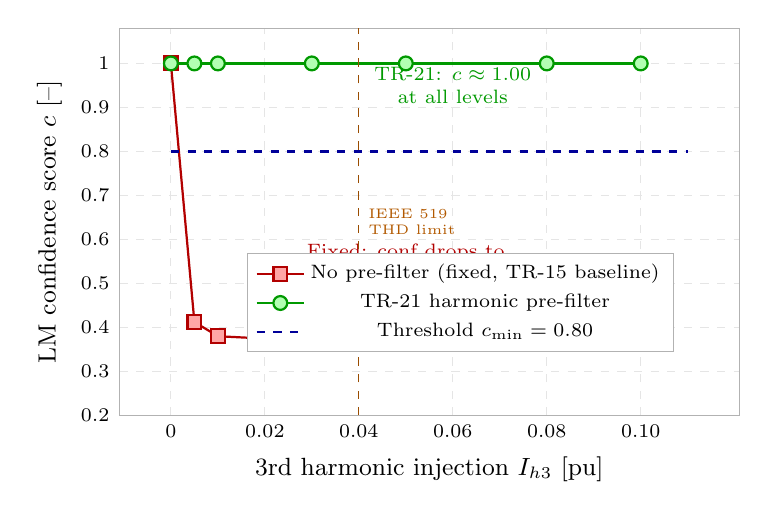
\begin{tikzpicture}
\begin{axis}[
  name          = confax,
  width         = 0.78\textwidth,
  height        = 6.5cm,
  ylabel        = {LM confidence score $c$ [--]},
  ylabel style  = {font=\small},
  xlabel        = {3rd harmonic injection $I_{h3}$ [pu]},
  xlabel style  = {font=\small},
  ymin=0.20, ymax=1.08,
  ytick         = {0.2, 0.3, 0.4, 0.5, 0.6, 0.7, 0.8, 0.9, 1.0},
  yticklabel style={font=\scriptsize},
  xtick         = {0, 0.02, 0.04, 0.06, 0.08, 0.10},
  xticklabels   = {0, 0.02, 0.04, 0.06, 0.08, 0.10},
  xticklabel style={font=\scriptsize},
  legend style={at={(0.55, 0.42)}, anchor=north,
                font=\scriptsize, draw=gray!60},
  grid          = major,
  grid style    = {gray!20, dashed},
  tick style    = {draw=none},
  axis line style={gray!60},
  mark size=2.5pt,
]

% Fixed correction (no harmonic filter): confidence collapses with I_harm
\addplot[red!70!black, thick, mark=square*,
         mark options={fill=red!35}]
  coordinates {
    (0.000, 1.0000)
    (0.005, 0.4124)
    (0.010, 0.3801)
    (0.030, 0.3693)
    (0.050, 0.3684)
    (0.080, 0.3681)
    (0.100, 0.3680)
  };
\addlegendentry{No pre-filter (fixed, TR-15 baseline)}

% TR-21 (harmonic pre-filter): confidence remains at 1.0
\addplot[green!60!black, thick, mark=*,
         mark options={fill=green!30}]
  coordinates {
    (0.000, 1.0000)
    (0.005, 1.0000)
    (0.010, 1.0000)
    (0.030, 1.0000)
    (0.050, 1.0000)
    (0.080, 1.0000)
    (0.100, 1.0000)
  };
\addlegendentry{TR-21 harmonic pre-filter}

% Confidence threshold at 0.80
\addplot[blue!60!black, thick, dashed, mark=none, domain=0:0.11, samples=2]
  ({x}, {0.80});
\addlegendentry{Threshold $c_{\min}=0.80$}

% ---- Annotations -------------------------------------------------------
\node[font=\scriptsize, red!70!black, align=center]
  at (axis cs:0.050, 0.52)
  {Fixed: conf drops to\\$\approx 0.37$ at any\\non-zero $I_{h3}$};
\draw[-latex, red!50!black, thin]
  (axis cs:0.050, 0.48) -- (axis cs:0.030, 0.40);

\node[font=\scriptsize, green!60!black, align=center]
  at (axis cs:0.060, 0.95)
  {TR-21: $c \approx 1.00$\\at all levels};

% ENTSO-E THD limit annotation (THD 5% ≈ I_h3 ≈ 0.04 pu for 3rd dominant)
\draw[orange!60!black, dashed, thin]
  (axis cs:0.040, 0.20) -- node[right, font=\tiny, orange!70!black, align=left]
    {IEEE 519\\THD limit}
  (axis cs:0.040, 1.08);

\end{axis}
\end{tikzpicture}
